\section{Image Scanning Microscopy}

Modern biological and biomedical research frequently demands the ability to image
microscopical structures, from one micrometer bacteria to amino acids in the nanometer scale. Optical microscopy has long been
the workhorse of such investigations, owing to its non-invasive nature and compatibility
with live specimens. Yet imaging at this scale is far from straightforward: two
fundamental requirements, \textit{high contrast} and \textit{high resolution}, are
each difficult to achieve and often stand in tension with one another. Moreover, conventional microscopy falls short under the micrometer scale, thus being incapable of observing structures such as viruses or proteins.

\subsection{Fluorescence Microscopy and the Diffraction Limit}

Fluorescence microscopy addresses the contrast challenge by exploiting the phenomenon of fluorescence: certain molecules (fluorophores) absorb excitation light at a shorter wavelength and re-emit it at a longer, less energetic wavelength. By selectively labelling specific cellular structures with fluorescent markers, one can visualize components of interest against a dark background with high specificity, effectively filtering out the rest of the sample. A widefield fluorescence microscope routes a laser excitation beam through an objective lens onto the specimen; the emitted fluorescent light is then separated from the excitation by a dichroic mirror and emission filter, and collected by a detector to form an image.

Resolution, however, is fundamentally bounded by the wave nature of light. A lens cannot focus an electromagnetic beam to an infinitely small spot. Instead, each point in the sample is imaged as a diffuse blob known as the \textit{Point Spread Function} (PSF). The width of the PSF determines the smallest resolvable feature: two emitters closer together than the PSF width are indistinguishable. This is formalized by the \textit{Abbe diffraction limit}, which states that the minimal resolvable distance $d$ satisfies
\begin{equation}
    d = \frac{\lambda}{2 \, \mathrm{NA}} = \frac{\lambda}{2 n \sin(\theta)}
    \approx 200\text{--}250 \; \text{nm},
\end{equation}
where $\lambda$ is the emission wavelength, $\mathrm{NA}$ is the numerical aperture of the objective, $n$ is the refractive index of the immersion medium, and $\theta$ is the half the angle of the acceptance cone. 

Equivalently, in the frequency domain, the \textit{Optical Transfer Function} (OTF) acts as a low-pass filter, suppressing spatial frequencies beyond a cutoff determined by the numerical aperture.

The consequence is that widefield fluorescence microscopy is limited to observe a surface of roughly a quarter of a micrometer, translating in the need of image reconstruction pipelines.

\subsection{Confocal Laser Scanning Microscopy}

The \textit{Confocal Laser Scanning Microscope} (CLSM) improves upon widefield imaging by replacing camera-based wide-area detection with a point-by-point scanning strategy. A focused laser beam is raster-scanned across the specimen using galvanometric mirrors; at each scan position $\mathbf{x}_s$, the emitted fluorescence passes back through the objective and is focused through a small \textit{pinhole} aperture onto a detector (for example a photodiode), which records a single photon-count value. The pinhole rejects anything that os out of focus, which has two advantages: optical sectioning (the ability to reconstruct thin focal planes within a thick specimen) and, when the pinhole is closed down, a modest improvement in lateral resolution beyond the Abbe limit by up to a factor of $\sqrt{2}$.

These gains come at a cost. Closing the pinhole necessarily discards a large fraction of the collected photons, severely reducing the signal-to-noise ratio (SNR), which leads to a situation that is never optimal: a wide pinhole recovers photon counts but degrades both sectioning and resolution, while a narrow pinhole improves spatial quality at the expense of a dim, noisy image. 

\subsection{Image Scanning Microscopy: Concept and Data Structure}

\textit{Image Scanning Microscopy} (ISM) resolves the CLSM trade-off by replacing the single-element detector with a two-dimensional \textit{Single-Photon Avalanche Diode (SPAD) array}. The array, approximately $1.4$ Airy Units, is centred on the optical axis. For each scan position $\mathbf{x}_s = (x_s, y_s)$, rather than integrating all arriving photons into one number, every pixel $\mathbf{x}_d = (x_d, y_d)$ of the detector array records its own photon count independently. A complete ISM acquisition therefore produces a \textit{four-dimensional dataset} $i(\mathbf{x}_s \mid \mathbf{x}_d)$, consisting of $(N_x \times N_y)$ micro-images (one per scan point), each of which is a small image of the sample as seen by a particular detector element. Equivalently, one may reorganize the same data as $N_\mathrm{ch}$ scanned images (one per detector pixel). This high-dimensional dataset carries substantially more spatial information than a conventional confocal acquisition and is a defining feature of the ISM modality \cite{zunino_open-source_2023}.

\subsection{Forward Model and the Inverse Problem}

The image formation process in fluorescence microscopy is well described as a \textit{linear shift-invariant} (LSI) system. The observed image is the convolution of the unknown fluorophore distribution $\mathbf{u} \in \mathbb{R}^N_+$ with the system's PSF $h$, corrupted by Poisson noise $\mathcal{P}$: 
\begin{equation} 
    \mathbf{y} = \mathcal{P}(\mathbf{h} * \mathbf{u}) = \mathcal{P}(\mathbf{A}\mathbf{u}), 
\end{equation} where $\mathbf{A} \in \mathbb{R}^{N \times N}$ is the Toeplitz matrix computing the convolution with the PSF. In CLSM the PSF is a product of the excitation PSF and the effective detection PSF shaped by the pinhole. 

In the ISM setting, the forward model generalizes to a family of $d$ equations 
\begin{equation} 
    \mathbf{y}_d = \mathcal{P}(\mathbf{h}_d * \mathbf{u}) = \mathcal{P}(\mathbf{A}_d \mathbf{u}), \qquad d = 1, \ldots, 25, 
\end{equation} 
where $\mathbf{y}_d \in \mathbb{N}^N$ is the measured image from detector $d$ with $p = n_1 \times n_2$ pixels, $\mathbf{u} \in \mathbb{R}_+^N$ is the unknown object, $\mathbf{A}_d \in \mathbb{R}^{N \times N}$ is the Toeplitz matrix to compute the convolution with the PSF $h_d$, and $\mathcal{P}$ is the Poisson noise.

Optical aberrations such as spherical aberration, astigmatism, and coma are common sources of PSF distortion in fluorescence microscopy, arising from refractive index mismatches, intentional depth encoding, or element misalignment. As illustrated by figure \ref{fig:ismexamples}, these aberrations manifest as characteristic deformations in both the detector offset patterns and the reconstructed PSF shapes, degrading spatial resolution and image quality. Accurately modeling and correcting for these effects is therefore essential for reliable reconstruction in any computational microscopy pipeline.

\begin{figure}[h]
  \centering
  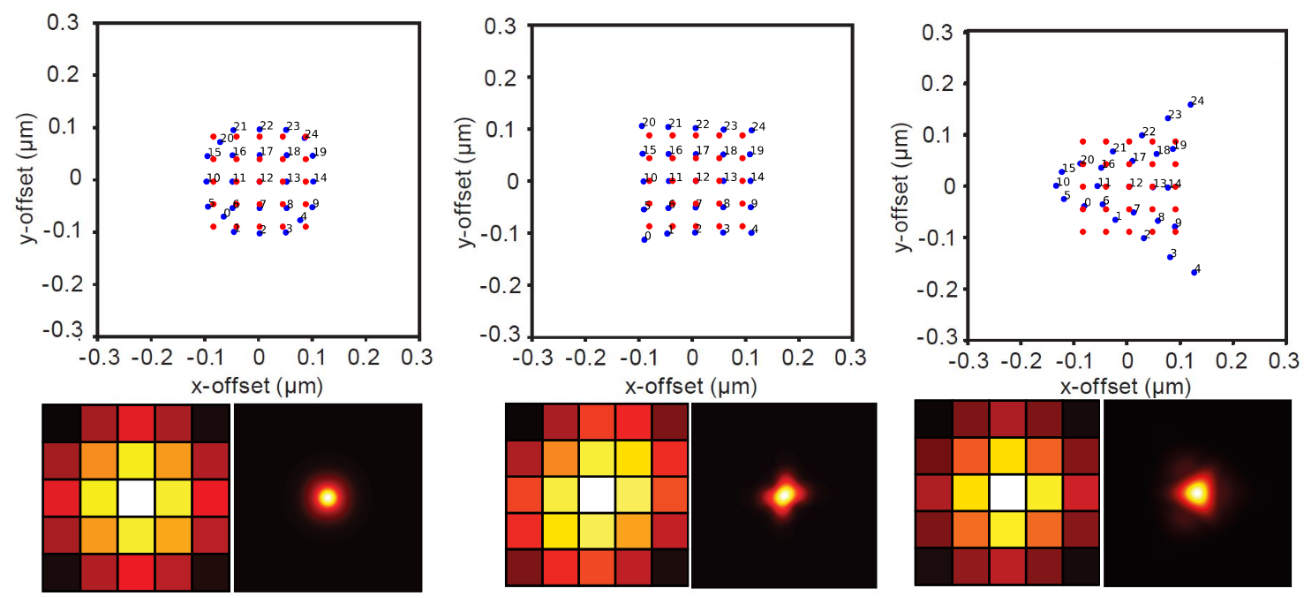
\includegraphics[width=.8\linewidth]{images/ismexamples.png}
  \caption{Aberrations examples on ISM.}
  \label{fig:ismexamples}
\end{figure}

\subsection{From Microscopy to Tomography}

The inverse problem structure of ISM shares mathematical parallels with that of Computed Tomography, discussed in the following section. In both cases, the objective is to recover an unknown spatial distribution from a collection of indirect, noisy measurements related to it through a linear forward operator. In ISM the forward operator is a convolution (a consequence of the LSI imaging model), while in CT it is the Radon transform (a consequence of straight-line X-ray propagation). Both are compact linear operators whose inversion is ill-posed and requires regularisation. Moreover, just as ISM acquires multiple shifted views of the same object, CT acquires projections from multiple angles with each angular view illuminating a different set of line integrals through the target. 

Both settings exemplify the broader programme of computational imaging, in which the design of the acquisition, the modelling of the forward physics, and the inversion algorithm are optimized to extract the maximum information about an object from measurements that are always finite, incomplete, and noisy.

\paragraph{Sources}

The list of sources for this section follow:
\begin{itemize}
    \item Slides \textit{"Image Scanning Microscopy: from forward to inverse problem formulations"}, authored by Luca Calatroni, Lisa Cuneo, and Giuseppe Vicidomini;
    \item A. Zunino et al., "Open-source tools enable accessible and advanced image scanning microscopy data analysis", Nature Photonics volume 17, pp 457–458 (2023) \cite{zunino_open-source_2023};
    \item A. Zunino et al., "Structured detection for simultaneous super-resolution and optical sectioning in laser scanning microscopy", Nature Photonics volume 19, pp 888–897 (2025) \cite{zunino_structured_2025};
    \item B. Richard and E. Wolf, Electromagnetic diffraction in optical systems II, Proceedings of the Royal Society of London. A. Mathematical and Physical Sciences (1959) \cite{richards_electromagnetic_1959};
    \item Y. Liu, V. Stergiopoulou et al, "Revisiting PSF models: unifying framework and high-performance implementation", arxiv DOI, (2025) \cite{liu_revisiting_2025};
    \item F. Fersini et al, Wavefront estimation through structured detection in laser scanning microscopy, Biomed. Opt. Express (2025) \cite{fersini_wavefront_2025}.
\end{itemize}